
\documentclass[ms.tex]{subfiles}
\begin{document}

\section{Discussion and Conclusions}
\label{sec:conclusions}

% fig 11
\begin{figure*}
\centering
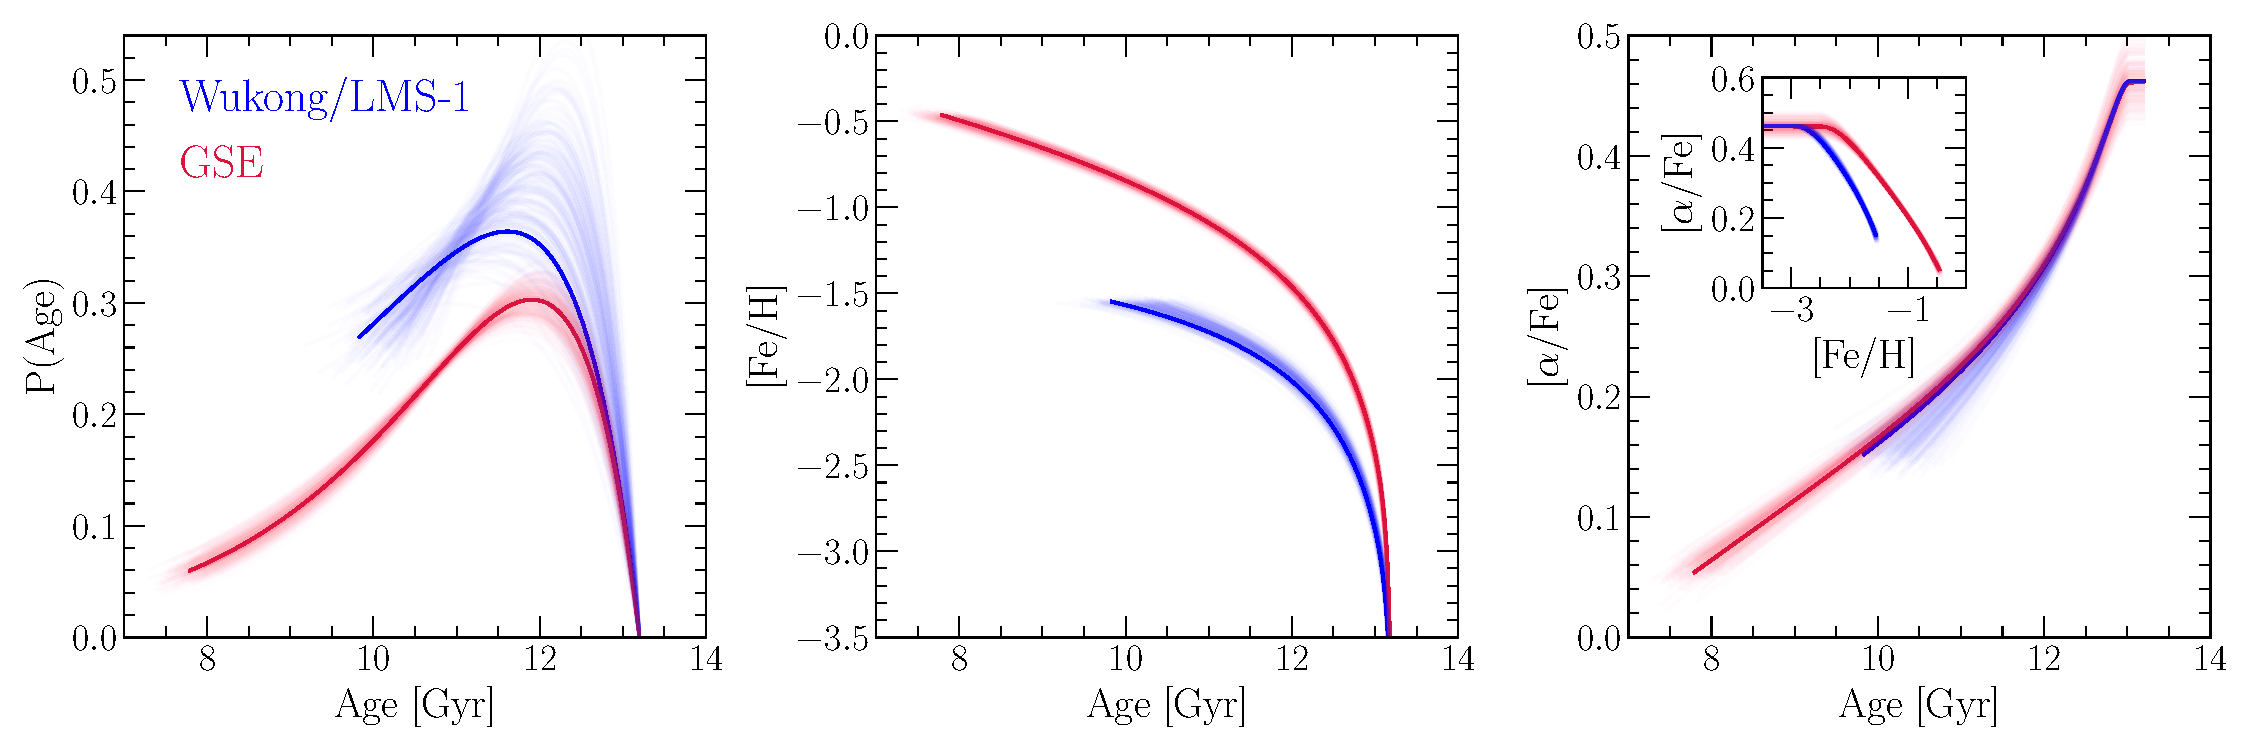
\includegraphics[scale = 0.45]{gse_wukong_comparison.pdf}
\caption{
A comparison of our best-fit models for GSE (red) and Wukong/LMS-1 (blue): the
age distributions (left), the age-\feh~relations (middle) and age-\afe~relations
(right).
The inset in the right hand panel shows the tracks in the~\afe-\feh~plane.
In all panels, we subsample 200 additional parameter choices from our Markov
chains and plot the predictions as high transparency lines to provide a sense
of the fit uncertainty.
Due to the lack of age information for Wukong/LMS-1, the centroid of the age
distribution is determined by our assumption that star formation began 13.2
Gyr ago (see discussion in~\S~\ref{sec:mocks:fiducial}).
}
\label{fig:comparison}
\end{figure*}

We use statistically robust methods to derive best-fit parameters of
one-zone GCE models for two disrupted dwarf galaxies in the Mily Way stellar
halo: GSE~\citep{Belokurov2018, Helmi2018}, and Wukong/LMS-1~\citep{Naidu2020,
Naidu2022, Yuan2020}.
We fit both galaxies with an exponential accretion history
(see~\S~\ref{sec:mocks}), deriving e-folding timescales and durations of star
formation of~$(\tau_\text{in}, \tau_\text{tot}) \approx (1~\text{Gyr},
5.4~\text{Gyr})$ for GSE and~$(\tau_\text{in}, \tau_\text{tot}) \approx
(3.1~\text{Gyr}, 3.4~\text{Gyr})$ for Wukong/LMS-1 (we refer to table
\ref{tab:results} for exact values).
These differences in evolutionary parameters are qualitatively consistent with
predictions from hydrodynamical simulations~\citep[e.g.,][]{GarrisonKimmel2019}
and semi-analytic models of galaxy formation~\citep[e.g.,][]{Baugh2006,
Somerville2015a, Behroozi2019}.
\par
Quantitatively, we arrive at a longer duration of star formation than
\citet{Gallart2019}, who derived an age distribution for GSE by analysing its
CMD according to the method described in~\citet{Dolphin2002} and found a
median age of 12.37 Gyr.
Consistent with their results,~\citet{Vincenzo2019} infer a sharply declining
infall history with a timescale of~$\tau_\text{in} = 0.24$ Gyr.
However, the star-by-star age measurements provided by H3~\citep{Conroy2019}
suggest that GSE's SFH was more extended (see Fig.~\ref{fig:gse}).
The peak of the age distribution is near~$\sim$11 Gyr (Fig.~\ref{fig:gse}),
consistent with Feuillet et al.'s~\citeyearpar{Feuillet2021} results
from~\gaia~\citep{Gaia2016} and APOGEE~\citep{Majewski2017}.
Consequently, we deduce a higher value of~$\tau_\text{in}$ of~$1.01 \pm 0.13$
Gyr.
If its first infall into the Milky Way halo was~$\sim$10 Gyr ago
\citep[e.g.,][]{Helmi2018, Bonaca2020}, then depending on exactly how long ago
it started forming stars, the duration of star formation we derive
($\tau_\text{tot} = 5.4$ Gyr) implies that GSE formed stars for~$\sim$$1.5 - 2$
Gyr after its first infall.
\par
To our knowledge, this is the first detailed modelling of multi-element stellar
abundances in Wukong/LMS-1.
Wukong/LMS-1 experienced a more extended accretion history
($\tau_\text{in} = 3.08^{+3.19}_{-1.16}$ Gyr), but the duration of star
formation was~$\sim$2 Gyr shorter than in GSe.
If they started forming stars around the same time, then Wukong/LMS-1 was
quenched at approximately the time of GSE's first infall.
However, our sample includes no age information for Wukong/LMS-1, so the
centroid of the age distribution is a prediction of our model as opposed to an
empirical constraint.
We find no statistically significant evidence of IMF variability or
metallicity-dependent Fe yields comparing GSE and Wukong/LMS-1.
A pathway to investigate this hypothesis further and potentially pin down the
yield-outflow degeneracy as well (see discussion in
Appendix~\ref{sec:degeneracy}) is to perform a hierarchical analysis of a
sample of galaxies where the yields are free parameters but are required to be
the same for all systems.
\par
Although these models are statistically good descriptions of our GSE and
Wukong/LMS-1 data, they are simplified in nature.
In particular, we have assumed a linear relation between the gas supply and the
SFR while empirical results would suggest a non-linear relation
\citep[e.g.,][]{Kennicutt1998, Kennicutt2012, delosReyes2019, Kennicutt2021}.
We have also taken a constant outflow mass-loading factor~$\eta$, when in
principle this parameter could vary with time as the potential well of the
galaxy deepens as in, e.g.,~\citet{Conroy2022}.
The primary motivation of these choices, however, is to provide proof of
concept for our fitting method with an example application to observations.
We reserve more detailed modelling of galaxies with both simple and complex
evolutionary histories for future work.
\par
Our method is built around a likelihood function which requires no binning of
the data (Eq.~\ref{eq:likelihood}) and has two central features.
First, the likelihood of observing some datum~$\script{D}_i$ must be
marginalized over the entire evolutionary track~\script{M}.
This requirement arises due to measurement uncertainties: for any given datum,
it is impossible to know where on the track the observation truly arose from,
and mathematically accounting for this requires considering all pair-wise
combinations between~\script{M} and~\script{D}.
Second, the likelihood of observing a datum~$\script{D}_i$ given a point on
the evolutionary track~$\script{M}_j$ must be weighted by the SFR at that time
in the model, simultaneously folding in any selection effects introduced by the
survey.
This requirement arises because an observed star is proportionally more likely
to have been sampled from an epoch of a galaxy's history in which the SFR was
large and/or if the survey designed is biased toward certain epochs.
\par
We establish the accuracy of our method by means of tests against mock data,
demonstrating that the known evolutionary parameters of subsampled input models
are accurately re-derived across a broad range of sample sizes
($N = 20 - 2000$), abundance uncertainties ($\sigma_\text{[X/Y]} = 0.01 - 0.5$),
age uncertainties ($\sigma_{\log_{10}(\text{age})} = 0.02 - 1$) and the
fraction of the sample with age information ($f_\text{age} = 0 - 1$; see
discussion in~\S~\ref{sec:mocks}).
The fit precision of the inferred parameters generally scales with sample size
as~$\sim$$N^{-0.5}$.
We demonstrate that evolutionary timescales can theoretically be derived with
abundances alone, but in practice age information helps reduce the effect of
systematic differences between the data and model, improving both the
accuracy and the precision.
Our likelihood function requires no binning of the data, and we derive it
in Appendix~\ref{sec:likelihood} assuming only that the model predicts an
evolutionary track of some unknown shape in the observed space.
It should therefore be applicable to one-zone models of any parametrization as
well as easily extensible to other astrophysical models in which the chief
prediction is a track of some form (e.g., stellar streams and isochrones).
\par
Having provided proof of concept for our method, a promising direction for
future work is to apply it to a much broader sample of disrupted dwarf galaxies
in the Milky Way stellar halo to take a ``chemical census'' of the accreted
systems.
This approach is also of interest to authors seeking to derive quenching
times (i.e., the lookback time to when star formation stopped) for intact and 
disrupted dwarf galaxies.
At present, the most reliable method to empirically determine a dwarf galaxy's
quenching time is via a direct reconstruction of its SFH through some method,
such as analysing its CMD~\citep[e.g.,][]{Sohn2013, Weisz2015}.
Consequently, the most precise SFH measurements are for nearby systems with
resolved stars, a considerable limitation even with modern instrumentation.
To our knowledge, there are only four quenched galaxies outside of the Milky
Way subgroup with well-constrained SFHs: Andromeda II, Andromeda XIV
\citep{Weisz2014a}, Cetus~\citep{Monelli2010a} and Tucana~\citep{Monelli2010b}.
Some authors have connected quenching timescales to observed galaxy properties
in N-body simulations (e.g.,~\citealp*{Rocha2012};~\citealp{Slater2013,
Slater2014, Phillips2014, Phillips2015, Wheeler2014}), but unfortunately
simulation outcomes are strongly dependent on the details of the adopted
sub-grid models~\citep[e.g.,][]{Li2020} as well as how feedback and the grid
itself are implemented~\citep{Hu2022}.
Our results suggest that chemical abundances can provide valuable additional
information for these methods.
% Our results suggest that the duration of star formation can instead be inferred
% from elemental abundance alone, though having~\textit{some} age information can
% significantly improve the precision of the fit.
% While this is theoretically possible, we demonstrate in~\S~\ref{sec:h3:gse}
% below that the exclusion of age information from the fit to our GSE sample
% produces significantly different results for evolutionary timescales.
% These discrepancies indicate that age information in some form is more
% important in practice than our proof of concept would suggest.
\par
% This method could have a strong impact in deriving SFHs and quenching times for
% dwarf galaxies.
However, with current instrumentation, spectroscopic measurements of
multi-element abundances in dwarf galaxies are limited to the local group
\citep[e.g.,][]{Kirby2011, Kirby2020}, and sample sizes are small even for
these relatively nearby systems.
Larger sample sizes could potentially be achieved with a high
angular resolution integral field unit such as the Multi Unit Spectroscopic
Explorer~\citep[MUSE;][]{Bacon2014}.
Alternatively, photometry is more conducive to larger sample sizes due to the
lower observational overhead, and the MDF can still be constrained using the
CMD~\citep[e.g.,][]{Lianou2011}.
One possibility is to forward-model the CMDs of dwarf galaxies using the SFHs
and MDFs predicted by one-zone GCE models, simultaneously constraining both
quantities photometrically.
% In some cases, narrow-band imaging can also provide worthwhile constraints on
% the MDF~\citep{Fu2022}, particularly when combined with machine learning
% algorithms trained on spectroscopic data~\citep{Whitten2011}.
The high angular resolution of the James Webb Space Telescope
\citep[JWST;][]{Gardner2006} should provide a considerable increase in the
number of resolved stars in nearby galaxies, making it a promising instrument
to pursue this potential pathway.
Farther in the future, the upcoming Nancy Grace Roman Space Telescope
(\citealp{Spergel2013, Spergel2015}; formerly WFIRST) will revolutionize
stellar populations in nearby galaxies.
In the era of next-generation telescopes, statistically robust methods such as
the one detailed in this paper will be essential to deduce the lessons the
community can learn about dwarf galaxy evolution.

\end{document}
